
\section{Métodologia de pruebas} 

Como metodología de pruebas para el proceso haremos uso 
de \href{https://owasp.org/www-pdf-archive/OWASP_Application_Security_Verification_Standard_4.0-en.pdf}{OWASP Application Security Verification Standard (ASVS) 4.0} 
que proporciona una base para probar los controles técnicos de seguridad de las aplicaciones web. El proyecto clasifica
 los distintos controles en tres niveles. En este caso cubriremos todos los controles incluidos en el \textbf{nivel 2}.

 Para abordar el proceso de pentesting los dividiremos en las fase definidas en el 
 apartado 2.1.2, para la ejecución del proceso de pentesting ejecutaremos todas las fases menos la 
 de explotación y postexplotación.tación y Postexplotación.

\textbf{Alcance y términos de la prueba de intrusión.}\\
 Para cada una de las aplicaciones crearemos un documento definición del plan de pruebas de seguridad donde se
detallará toda la información de las pruebas de seguridad a ejecutar.
\textbf{Recolección de información.}\\
En esta fase ejecutaremos el análisis estático de dependencias y generaremos un reporte del análisis estático de código. Los resultados del 
análisis estático servirán como base para crear un plan de pruebas para el análisis dinámico.
\textbf{Análisis de vulnerabilidades.}\\
En esta fase ejecutaremos el análisis dinámico de código a partir del plan de pruebas generado con la información obtenida en la fase anterior.
En esta fase ejecutarán dos veces el escáner de análisis dinámico con distinto número de reglas:
\begin{itemize}
    \item \textbf{Escanér regular:} Para descubrir todas las posibles rutas validados debajo de los dominios 
    a evaluar a partir del plan de pruebas definido con los datos de la fase anterior.
    \item \textbf{Escáner Comleto:} A partir del escáner regular, para obtener el reporte definitivo después 
    de revisar los errores encontrados para descartar los no relevantes y los falsos positivos.
\end{itemize}
\textbf{Generación de informes}\\
Como resultado el proceso de ejecución de las pruebas de seguridad generaremos los siguientes documentos.
\begin{itemize}
    \item Definición del plan de pruebas de seguridad.
    \item Reporte análisis estático de código.
    \item Plan pruebas para el análisis dinámico.
    \item Reporte análisis dinámico
    \item Informe resultado ejecución pruebas de seguridad
\end{itemize}


\section{Infraestructura de pruebas} 
Como entorno de pruebas para la ejecución de los análisis de código; haremos uso de una máquina física y de un contenedor 
de Docker con la siguientes características y herramientas instaladas en cada una de ellas:

\begin{table}
    \begin{center}
      \caption{Parámetros línea comandos dependency-check}
      \label{tab:Infraestructura de pruebas}
      \begin{tabular}{c|c|c}
        \textbf{Características} & \textbf{Máquina física} & \textb{Contenedor}\\
        \hline
        Sistema Operativo & Windows 10 Pro & Debian GNU/Linux 10 (buster)\\ 
        Herramientas & OWASP Zap 2.10
        Dependency-check
        SonarScaner 4.6.2
         & SonarQube 8.2
         PostGresSQL 13.3 \\ 
      \end{tabular}
    \end{center}
  \end{table}

Para levantar el contenedor podemos hacer uso de dockercompose incluido en la carpeta \textbf{"entornoPrueba"} dentro de 
las \href{https://github.com/M0l1n3ta/PFG/tree/master}{fuentes de proyecto}

Para levantar el entorno ejecutamos:
\begin{verbatim}
    docker-compose up
\end{verbatim}

\begin{figure}[h!]  
    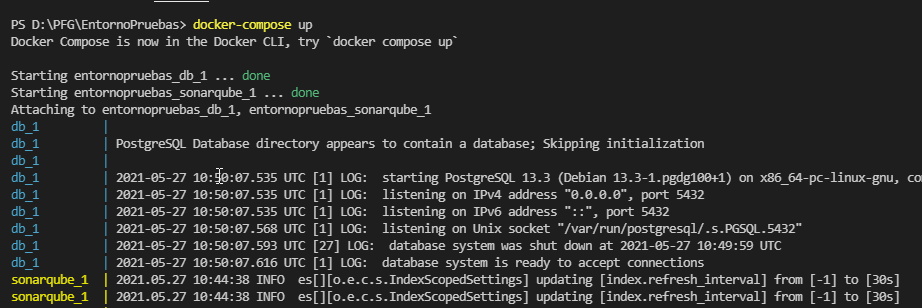
\includegraphics[width=\linewidth]{./imagenes/04_DockerCompose_UP.png}
    \caption{Docker compose up}  
    \label{fig:4}
\end{figure}

Una vez que se vena las siguientes líneas en el log:
\begin{figure}[h!]  
    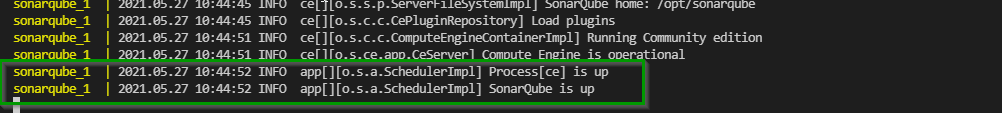
\includegraphics[width=\linewidth]{./imagenes/05_SonarQubeServerRunning.png}
    \caption{SonarQube server running}  
    \label{fig:5}
\end{figure}

Podremos acceder a la página de SonarQube en la url \href{http://localhost:9000}{http://localhost:9000}
\begin{figure}[h!]  
    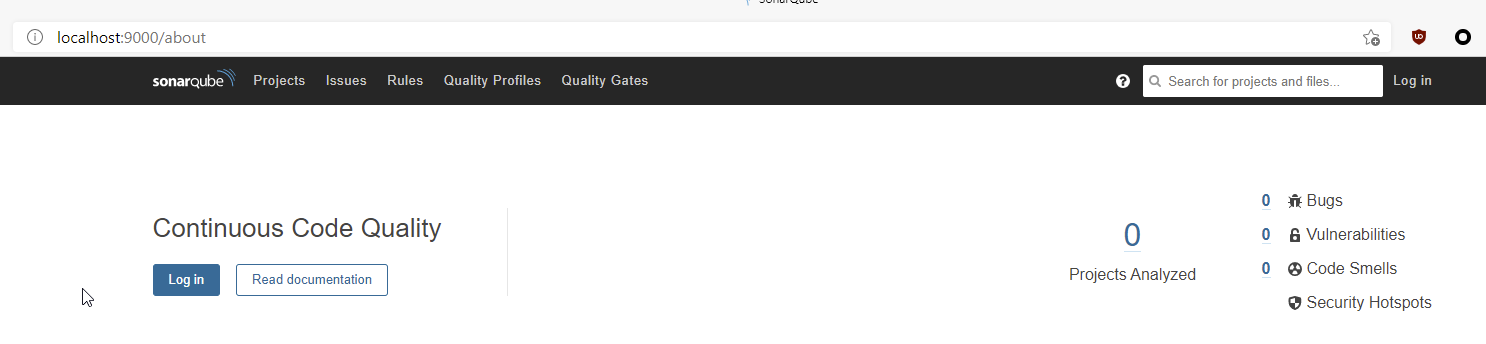
\includegraphics[width=\linewidth]{./imagenes/06_SonarQubeServer_Webpage.png}
    \caption{SonarQube portal}  
    \label{fig:6}
\end{figure}
Docker Compose SonarQube:
\begin{listing}[ht]
    \inputminted{yaml}{./EntornoPruebas/SonarQube_8.2/docker-compose.yml}
    \caption{Example from external file}
    \label{listing:3}
  \end{listing}
